\documentclass[a4paper,12pt]{report}

\usepackage{cmap}
\usepackage[T2A]{fontenc}
\usepackage[utf8]{inputenc}
\usepackage[russian]{babel}
\usepackage{amsmath,amsfonts,amssymb}
\usepackage{graphicx}
\usepackage{sidecap}
\usepackage{wrapfig}
\usepackage{indentfirst}

\begin{document} 

\begin{titlepage} 

\begin{center} 

\large Федеральное государственное автономное образовательное учреждение высшего образования «Санкт-Петербургский государственный электротехнический университет «ЛЭТИ» им. В.И. Ульянова (Ленина)»\\
кафедра Вычислительной техники\\[5cm] 

\huge ОТЧЕТ\\ по лабораторной работе № 10\\[0.5cm] 
\large <<Кольцевые списки>>\\[3.7cm]

\begin{minipage}{1\textwidth}
    \begin{flushleft}
        \emph{Автор:} Стукен В.А.\\
        \emph{Группа:} 2307\\
        \emph{Факультет:} ФКТИ\\
        \emph{Преподаватель:} Аббас Саддам Ахмед\\
    \end{flushleft}
\end{minipage}

\vfill

Санкт-Петербург, 2023\\
{\large \LaTeX}

\end{center}
\thispagestyle{empty}
\end{titlepage}

\section*{Задание(вариант 13)}
Для двусвязного кольцевого списка, насчитывающего 12 элементов, разработать подалгоритм и написать функцию перемещения «головы» в заданную позицию (перед элементом списка с указанным номером).
\section*{Постановка задачи и описание решения}
\par

Сначала задаем двусвязный кольцевой список (ф-ция init-list()), далее выводим полученный список(ф-ция print-list), далее просим пользователя ввести номер элемента, который станет головой списка(ф-ция move-head), выводим полученный список.

\section*{Описание переменных-функция main}
\begin{centering}
\resizebox{14cm}{!}{
    \begin{tabular}{|l|l|l|l|}
        \hline
        \textbf{№} & \textbf{Имя переменной} & \textbf{Тип} & \textbf{Назначение}\\
        \hline
        1 &  head   &  LHead* & Указатель на голову списка \\
        \hline
        2 &      first-node   & LNode* & Указатель на первый элемент списка\\ 
        \hline
        3 &      pos   & int & Позиция элемента, которую вводит пользователь\\ 
        \hline
        4 &      temp   & LNode* & Указатель на предыдущий элемент списка\\ 
        \hline
        
    \end{tabular}
}
\end{centering}
\section*{Примеры работы программы:}
\begin{figure}[ph]
    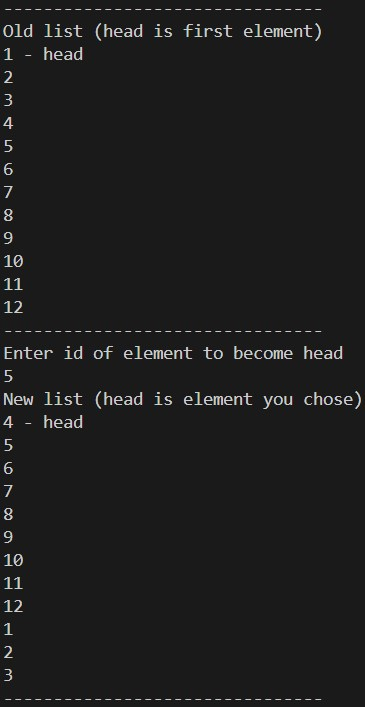
\includegraphics[width=0.7\textwidth]{ex1.jpg}
\caption{Пример 1}
\label{ris:image1}
\end{figure}
\begin{figure}[ph]
    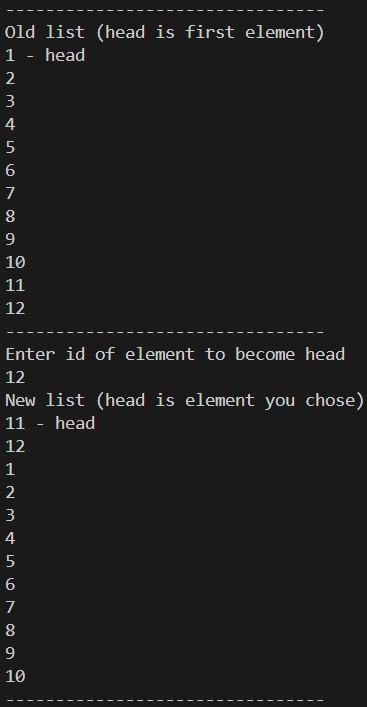
\includegraphics[width=0.7\textwidth]{ex2.jpg}
\caption{Пример 2}
\label{ris:image2}
\end{figure}




\begin{figure}[ph]
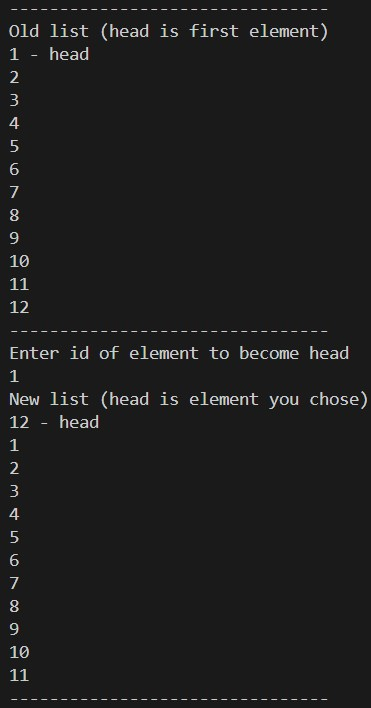
\includegraphics[width=0.7\textwidth]{ex3.jpg}
\caption{Пример 3}


\end{figure}


\newpage

\section*{Вывод}
В данной лабораторной работе научились работать с простейшими кольцевыми списками, выводить их элементы и т.д.
\end{document}